\section{Newton's Method}

\textbf{Needs} $f'(p_k)$ to exist.

We might have that:
\begin{itemize}
\item $f'$ is not available
\item $f'$ is expensive
\end{itemize}

We might choose to approximate:

\[
  f'(p_k) \approx \frac{f(p_{k-1})-f(p_{k-2})}{p_{k-1}-p_{k-2}}
.\]

This gives the secant method:

\begin{center}
  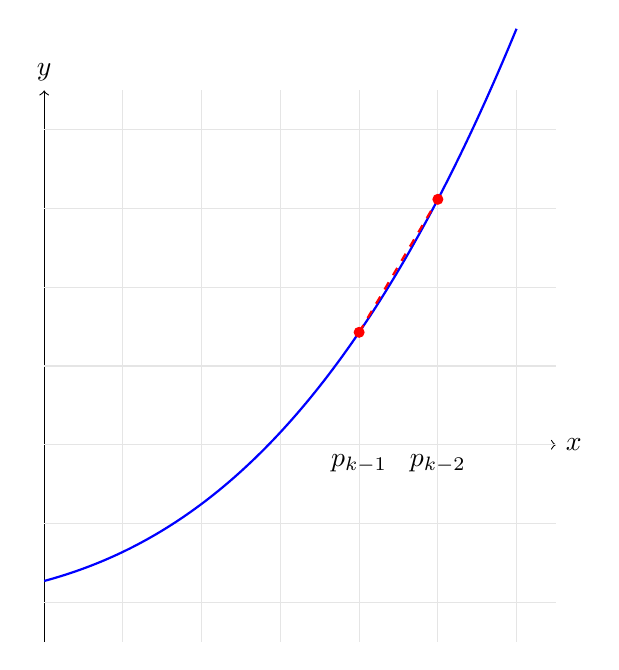
\begin{tikzpicture}[scale=1]
  % Axes
    \draw[->] (0,0) -- (6.5,0) node[right] {$x$};
    \draw[->] (0,-2.5) -- (0,4.5) node[above] {$y$};

  % Grid
    \foreach \x in {1,...,6} {
      \draw[gray!20] (\x,-2.5) -- (\x,4.5);
    }
    \foreach \y in {-2,-1,0,1,2,3,4} {
      \draw[gray!20] (0,\y) -- (6.5,\y);
    }

  % Labels for xticks
    \node[below] at (4,0) {$p_{k-1}$};
    \node[below] at (5,0) {$p_{k-2}$};

  % Function plot
    \draw[blue, thick, domain=0:6, samples=100, smooth, variable=\x] 
      plot ({\x}, {0.01*(\x + 3)^3 - 2});

  % Points
    \pgfmathsetmacro{\yA}{0.01*(4+3)^3 - 2} % = 0.01 * 343 - 2 = 3.43 - 2 = 1.43
    \pgfmathsetmacro{\yB}{0.01*(5+3)^3 - 2} % = 0.01 * 512 - 2 = 5.12 - 2 = 3.12
    \fill[red] (4,\yA) circle (2pt);
    \fill[red] (5,\yB) circle (2pt);

  % Secant line: from (4, \yA) to (5, \yB)
    \draw[red, dashed, thick] 
      (4,\yA) -- (5,\yB);

  % Optional: label the line
  % \node[anchor=south, red] at (4.5,{(\yA+\yB)/2}) 
  %   {\small $y = \frac{\yB - \yA}{1} (x - 4) + \yA$};

  \end{tikzpicture}
\end{center}

both newton's method and the secant method have the limitation that they may
diverge when the initial guess is not sufficiently close to the root. In 
bisection, we used the idea of bracketing the root at each step to ensure
convergence. 

\section{False Position}

If instead of considering a midpoint approximation for the root \newline
($\displaystyle p_k \approx p_0 + \frac{p_1 - p_0}{2}$), we consider a
secant approximation for the root (based on the endpoints of the interval).
This is called the \textbf{Method of False Position}.

\[
p_k \approx p_1 - f(p_1) \frac{p_1-p_0}{f(p_0)-f(p_1)}
.\]

\section{oops, skipped a bunch of pages}

\section{Error Analysis}

We want to be able to give a more precise description of how a method converges
to a the solution. For example, consider finding a root for the polynomial

\[
x^3 + 4x^2 - 10 = 0
.\]

with two different methods (A and B). Suppose that the errors produced by these 
methods are as given below.

\begin{table}[h]
    \centering
    \begin{tabular}{|c|c|c|}
        \hline
        & \textbf{Method A} & \textbf{Method B} \\
        \hline
        $|p - p_0|$ & 0.134769987 & 0.134769987 \\
        $|p - p_1|$ & 0.078276245 & 0.008103332 \\
        $|p - p_2|$ & 0.037310791 & 0.000003811 \\
        $|p - p_3|$ & 0.019771639 & 0.000000000 \\
        $|p - p_4|$ & 0.009940240 & \text{to all significant digits} \\
        \hline
    \end{tabular}
    \caption{Comparison of Methods A and B}
\end{table}

Notice that the error for method $A$ decreases by a constant factor (about 2)
at each iteration. For method $B$, the error drops off much more quickly. The
error at step $n$ is roughly proportional to the error at step $n-1$, squared.

\textbf{Both of these behaviours can be quantified.}

\noindent\defn Suppose $\{ p_n \}_{n=0}^\infty$ is a sequence that converges to $p$,
with $p_n \neq p$ for all $n$. If positive constants $\lambda$ and $\alpha$
exist with $\displaystyle \lim_{n\to\infty} \frac{|p_{n+1}-p|}{|p_n -p|^\alpha} = \lambda$
then $\{ p_n \}_{n=0}^\infty$ converges to $p$ of order $\alpha$, with asymptotic
error constant $\lambda$.

Notice that:
\begin{itemize}
\item a sequence with high order of convergence converges more rapidly than a
  sequence with a lower order.
\item the constant $\lambda$ affects the speed of convergence, but is not as
  important as the order ($\alpha$).
\item We want a large $\alpha$. $\alpha \geq 1$ is sufficient. \\
  If $\alpha = 0.5$, for example, then the error at $k$ is proportional
  to the square root of the error at $k-1$. This is not a good behaviour.
\end{itemize}

\subsection{Common Cases}

For different values of $\alpha$, we observe the following convergence behaviors:

\begin{itemize}
    \item $\alpha = 1$, $\lambda < 1$: Linearly convergent.
    \[ \bigEps_{n+1} \approx \lambda \bigEps_n \]
    
    \item $\alpha = 2$: Quadratically convergent.
    \[ \bigEps_{n+1} \approx \lambda \bigEps_n^2 \]
    
    \item $\alpha$ does not have to be an integer. For example, the secant method has:
    \[ \alpha = \frac{1+\sqrt{5}}{2} < 2. \]
\end{itemize}

\textbf{In order to truly understand the behaviour of a method, we need to
  find both the order and the asymptotic error constant.}

\section{Thm (2.7 of Text)}

Let $g\in C[a,b]$ s.t. $g(x) \in [a, b]$ for all $x \in [a, b]$.

Suppose, in addition, that $g'$ is continuous on $(a,b)$ and a constant
$0\leq k<1$ exists with $|g'(x)|\leq k$ for all $x\in (a,b)$.

If $g'(p) \neq 0$, then for any number $p_0$ in $[a,b]$ the sequence 

\[
  p_n = g(p_{n-1}) \text{ for } n\geq 1
.\]

converges only linearly to the unique fixed point $p$ in $[a,b]$.

\proof We know from the fixed point theorem that the sequence converges to $p$.
since $g'$ exists on $[a,b]$ we can apply the mean value theorem to g:

\[
\underbrace{g(p_n) - g(p)}_{p_{n+1} - p} = g'(\xi_n)(p_n - p)
.\]

where $\xi_n$ is between $p_n$ and $p$. Thus,

\[
  \frac{p_{n+1}-p}{p_n-p} = g'(\xi_n)
.\]

and fixed point iteration gives linear convergence with asymptotic error
constant $|g'(p)|$ whenever $g'(p) \neq 0$.

